\chapter{Distribution of directional extensions} \label{ch:distribution}

This chapter presents data on how many Chadic languages have each type of directional extension. In general, directional extensions are nearly twice as common in Chadic languages as they are in large cross-linguistic samples of languages. However, directional extensions are not evenly distributed across Chadic languages. There is a strong bias toward directional extensions in some branches, and a few subbranches show a bias against directional extensions. There is also an uneven distribution with regard to semantic types. Ventive directional extensions are by far the most common type and are found across all branches. In contrast, most other types of directional extensions are only found in Biu-Mandara languages. 

Section \ref{sec:diroverview} provides a brief overview of how frequently each type of directional extension appears in Chadic languages. The remainder of this chapter gives more details about the various types of directional extensions: ventive (Section \ref{sec:vent2}), itive (Section \ref{sec:itive2}), inward and outward (Section \ref{sec:bounded2}), upward and downward (Section \ref{sec:vertical2}) and `onto' and `under' (Section \ref{sec:onto2}). Naturally, many languages have more than one directional extension. The patterns of co-occurrence of directional extensions in particular languages are discussed in Section \ref{sec:co-occurrence}. Section \ref{sec:sumdir} is a brief conclusion.

The same morphemes that function as directional extensions also tend to have other functions. These functions are discussed in Chapter \ref{ch:functions}. This chapter only discusses the directional functions of these verbal extensions. 

\section{Overview} \label{sec:diroverview}

From a global perspective, \citet[277--283]{rossPseudocoordinationSerialVerb2021} finds directional morphology in 114 languages of a balanced sample of 325 languages (35\%). The Grambank sample of over 2,000 languages includes data on a grammatical feature of ``directional or locative morphological marking on verbs'' \citep{thegrambankconsortiumGrambankV12023}. Even by this broader definition, they find that only 38\% of languages have this feature (799 of 2,105 languages).

60 of the 91 Chadic languages in this study (65.9\%) have at least one type of directional extension. This is a significantly higher rate than that at which directional extensions are found in languages generally.\footnote{By binomial test, 60 of 91 is significantly higher than Ross' finding of 35\% cross-linguistically (p < 0.001) as well as being significantly higher than a null hypothesis of a random (50\%) distribution (p < 0.01).} However, directional extensions are not evenly distributed across the branches and subbranches of Chadic languages. Table \ref{tab:directionalsbybranch} shows the number of languages with and without directional extensions broken down by subbranch.\footnote{In Table \ref{tab:directionalsbybranch} and subsequent tables, the circles in the column labeled \% are pie charts in which the black portion represents the percentage of total languages in each row that have the feature under discussion.} 

%Table in tab:directionalsbybranch based on python script in Number file
\begin{table}
	\caption{Number of Chadic languages with a directional extension by subbranch}
	\label{tab:directionalsbybranch}
	\begin{tabular}{lrrc} % add l for every additional column or remove as necessary
		\lsptoprule
		Subbranch &  One or more &  	No directionals & \% \\
		\midrule
		West A            &   13 &  9 &  \bwpie{13}{9} \\
		West B            &    2 &   5 &  \bwpie{2}{5} \\
		Biu-Mandara Hurza &    2 &   0 &  \bwpie{2}{0} \\
		Biu-Mandara North &   25 &   2 &  \bwpie{25}{2} \\
		Biu-Mandara South &   12 &   1 &  \bwpie{12}{1} \\
		Masa North        &    2 &   0 &  \bwpie{2}{0} \\
		Masa South        &    1 &   1 &  \bwpie{1}{1} \\
		East A            &    2 &   3 &  \bwpie{2}{3} \\
		East B            &    1 &  10 &  \bwpie{1}{10} \\
		\midrule
		Total             &       60 &          31 &  \bwpie{60}{31} \\
		\lspbottomrule
	\end{tabular}
\end{table}

Biu-Mandara and Masa languages are the most likely to have a directional extension. Directional extensions are found in 39 of 42 Biu-Mandara languages and in three of four Masa languages (91\% overall).\footnote{By binomial test, this rate (42 of 46) is significantly higher (p < 0.001) than the rate at which directional exstensions are found in Chadic languages overall. The same result is found for the 39 of 42 Biu-Mandara languages that have a directional extension. The sample size for Masa languages is not large enough for statistical significance on its own.} Outside of Biu-Mandara and Masa languages, directional extensions are significantly less common, found in just 17 of 45 languages (37\%).\footnote{By binomial test, the rate of 17 of 45 is significantly lower than the overall rate of 64.8\% across the language family (p < 0.01).} Directional extensions are least common in East Chadic B (Guera region) languages, attested in only one of ten languages.

Of the 60 languages with a directional extension, most (44) have only one or two directional extensions, while 16 have three or more, as shown in Table \ref{tab:dirmorphs}. On the extreme end is \hyperref[dghw]{Dghwede} with 11 directional extensions attested, some with overlapping functions (Chapter \ref{ch:identifying2}, Section \ref{sec:portmanteau}). 

%Table created using Python script in file Number.ipynb
\begin{table}
	\caption{Directional extensions in Chadic languages}
	\label{tab:dirmorphs}
	\begin{tabular}{rr} % add l for every additional column or remove as necessary
		\lsptoprule
Number of directional & Number of \\
extensions & languages \\
\midrule
0  &	31 \\
1  &     31 \\
2  &     13 \\
3  &      3 \\
4  &      4 \\
5  &      4 \\
7  &      3 \\
8  &      1 \\
11 &      1 \\
		\lspbottomrule
	\end{tabular}
\end{table}


%4   &      1 \\
%5   &      1 \\
%15  &      1 \\
%117 &      1 \\

%The most common path expressed by a directional extension is ventive. Ventive directional extensions are attested in 46 languages, just over half of all of the languages in the dataset, as seen in Table \ref{tab:directionals}. Ventive directional extensions are found across all four branches of Chadic languages. The other seven types of directional extensions are only attested in Biu-Mandara and Masa languages with the exception of one marginal case of an itive extension in the East Chadic language \hyperref[kera]{Kera}. Itive directional extensions are the second most frequently attested, followed by the inward and outward extensions. Upward and downward extensions are less frequently attested, with downward extensions being more frequent than upward extensions. The `onto' extensions are as frequent as upward extensions, but `under' extensions are the rarest type.

%Table created using Python script in file Directionals.ipynb
%The following values are irrelevant as Dghwede is already counted for all types of directionality
%ITIVE.DOWN &     0 &            1 &     0 &     0 &      1 \\
%VENT.OUT   &     0 &            1 &     0 &     0 &      1 \\
%VENT.DOWN  &     0 &            1 &     0 &     0 &      1 \\
\begin{table}
	\caption{Directional extensions by directional meaning}
	\label{tab:directionals}
	\begin{tabularx}{\textwidth}{l Yrrr Y}
		\lsptoprule
	 & West (29)	&	Biu-M. (42)	&	Masa (4)	&	East (16)	&	Total (91)	\\
\midrule
VENT       &    15 &           26 &     3 &     3 &     47 \\
ITIVE      &     0 &           16 &     2 &     1 &     19 \\
INTO       &     0 &           16 &     0 &     0 &     16 \\
OUT        &     0 &           15 &     0 &     0 &     15 \\
UP         &     0 &            8 &     0 &     0 &      8 \\
DOWN       &     0 &           13 &     0 &     0 &     13 \\
ONTO       &     0 &            9 &     0 &     0 &      9 \\
UNDER      &     0 &            3 &     0 &     0 &      3 \\
		\lspbottomrule
	\end{tabularx}
\end{table}

All of the languages with three or more directional extensions are from the Biu-Mandara branch. So not only are Biu-Mandara languages more likely to have a directional extension, they also have more of them per language. Another way to understand the preference for directional extensions in Biu-Mandara languages is that of the 142 morphemes that have been identified as a directional extension, 117 of them are from Biu-Mandara languages. Biu-Mandara languages make up 46\% of the languages in the sample but have 82\% of the directional extensions. 

The bias toward directional extensions in Biu-Mandara correlates with a wider range of semantic types of directional extension. Table \ref{tab:directionals} shows how many languages in each branch have at least one of each semantic type of direction extensions. There is a sharp contrast between the many types of directional extensions attested in Biu-Mandara languages compared with other branches. Masa, West Chadic and East Chadic languages are mostly restricted to ventive extensions with the exception of three languages that have an itive extension. 

\section{Ventive directional extensions} \label{sec:vent2}

Ventive directional extensions are the most common type of directional extension. They are found in just over half of the 91 Chadic languages in the sample, as shown in Table \ref{tab:directionals} and broken down by subbranch in Table \ref{tab:ventive}. 

%Table in tab:ventive based on python script in Ventive file
\begin{table}
	\caption{Number of Chadic languages with a ventive extension}
	\label{tab:ventive}
	\begin{tabular}{lrrc}
		\lsptoprule
		Subbranch &  Ventive &  	No ventive & \% \\
		\midrule
West A            &       13 &          9  &  \bwpie{13}{9} \\
West B            &        2 &           5 &  \bwpie{2}{5} \\
Biu-Mandara Hurza &        2 &           0 &  \bwpie{2}{0} \\
Biu-Mandara North &       14 &          13 &  \bwpie{14}{13} \\
Biu-Mandara South &       10 &           3 &   \bwpie{10}{3} \\
Masa North        &        2 &           0 &   \bwpie{2}{0} \\
Masa South        &        1 &           1 &   \bwpie{1}{1} \\
East A            &        2 &           3 &   \bwpie{2}{3} \\
East B            &        1 &          10 &  \bwpie{1}{10} \\
\midrule
Total             &       47 &          44 &  \bwpie{47}{44} \\
		\lspbottomrule
	\end{tabular}
\end{table}

\begin{figure}
	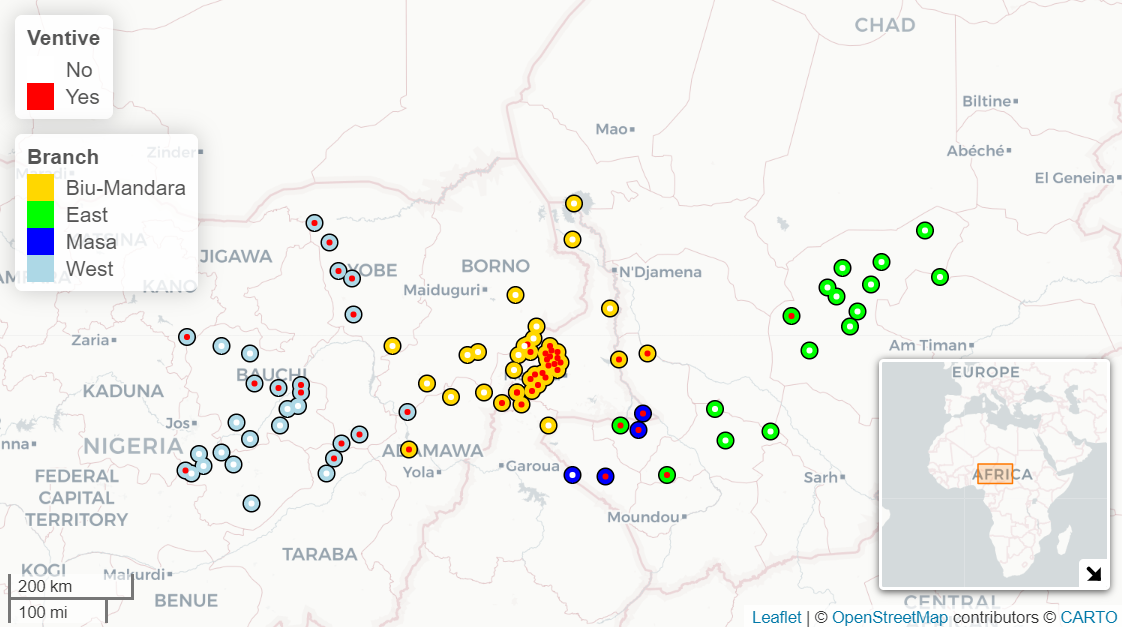
\includegraphics[width=\textwidth]{maps/ventive.png}
	\caption{Map of ventive directional extensions in Chadic languages}
	\label{fig:ventivemap}
\end{figure}



In the West branch, ventive extensions are the only attested type of directional extension and are found in 15 of the 29 West Chadic languages in the sample. Most of the examples of ventive extensions in West Chadic languages are from the West Chadic A group.\footnote{One additional West Chadic A language, \hyperref[beel]{Beele}, is said to have ventive extensions \citep[21]{schuhBoleTangaleLanguagesBauchi1978}, but it is not counted here since no examples are given to support the analysis.} Within the West Chadic B group, only two languages have evidence of a ventive extension. These are both part of the West B1 subgroup and are spoken in the northern part of Nigeria (Yobe State) in an area quite far from other West B languages. \citet[308]{schuhChadicCornucopia2017} states that there are no traces of directional extensions in West Chadic B2 or West Chadic B3.\footnote{\citet[]{schuhChadicCornucopia2017} uses the label \textit{West Chadic C} for West Chadic B3.} If this is correct, the distinction between West A and West B is even more stark than indicated in Table \ref{tab:ventive}. It is plausible that all West Chadic ventive directional extensions are cognate forms, but this cannot be extended to establish a historical relationship with ventive extensions in other branches (Chapter \ref{ch:diachrony}).

Among Biu-Mandara languages, 26 of 42 have a ventive extension (62\%). Ventive extensions are most common among the Biu-Mandara South subgroup (10 of 13). Within this subbranch, all six Dabaic languages have a ventive form that could be reconstructed as  $^\ast$\textit{-aha}. In the Biu-Mandara North subbranch, ventive extensions are not uncommon, found in 14 of 27 languages, but with a variety of forms. There is an areal dimension to the distribution of ventive extensions in North Biu-Mandara languages. As shown in the map in Figure \ref{fig:ventivemap}, there is a dense cluster of Biu-Mandara languages spoken in the area between the city of Maroua and the Mandara mountain range on the Cameroon-Nigerian border. The Biu-Mandara North languages spoken in this area all have a ventive extension. The North Biu-Mandara languages found to the west and north of this area do not have ventive extensions. 

Three of the four Masa languages in the sample have ventive extensions. The North Masa languages have similar suffixes featuring a palatal approximant, but the ventive extension \textit{-fi} in the South Masa language Herdé cannot be assumed to be a cognate form. 

Compared to other branches, there is a significant bias against ventive extensions in East Chadic languages with such morphemes attested in less than 20\% of languages (three of 16).\footnote{By binomial test, the rate of three of 16 is significantly lower than the rate of 47 of 91 languages (52\%) overall for all Chadic branches (p < 0.01).} Keeping in mind the limited data available for the East Chadic A group of languages (descriptions are available for only five of 15 languages), it appears that ventive extensions may be relatively common there compared to the East Chadic B subgroup (the easternmost cluster of Chadic languages) which stands out as having very few instances of ventive extensions attested (or any directional extensions at all). The two East Chadic A languages with directionals are spoken in the same geographical area as Masa languages, so language contact is a possible explanation for the appearance of directional extensions in these languages. This area is not far east of the dense cluster of Biu-Mandara languages with a ventive extension discussed above, as shown on the map in Figure \ref{fig:ventivemap}. 

\section{Itive directional extensions} \label{sec:itive2}

Itive directional extensions are almost exclusively found in Biu-Mandara and Masa languages, as seen in Table \ref{tab:itive}. They are attested in nearly 40\% of Biu-Mandara and Masa languages. No itive extensions are attested in West Chadic languages, and only one case has been identified in East Chadic languages. This strong correlation between subbranches and the presence of itive extensions essentially determines the geographic distribution of itive extensions as well, but it can be observed in the map in Figure \ref{fig:itivemap} that the Biu-Mandara languages spoken furthest north (the Kotoko-Buduma subgroup) do not have itive extensions.

%Data in tab:itive based on number from python script in Itive file
\begin{table}
	\caption{Numbers of Chadic languages with an itive extension}
	\label{tab:itive}
	\begin{tabular}{lrrc} % add l for every additional column or remove as necessary
		\lsptoprule
		Subbranch &  Itive &  	No itive & \% \\
		\midrule
West A            &      0 &        22 &  \bwpie{0}{22} \\
West B            &      0 &         7 &  \bwpie{0}{7}  \\
Biu-Mandara Hurza &      0 &         2 &  \bwpie{0}{2} \\
Biu-Mandara North &     12 &        15 &  \bwpie{12}{15} \\
Biu-Mandara South &      4 &         9 &  \bwpie{4}{9} \\
Masa North        &      2 &         0 &  \bwpie{2}{0} \\
Masa South        &      0 &         2 &  \bwpie{0}{2}  \\
East A            &      1 &         4 &   \bwpie{1}{4}  \\
East B            &      0 &        11 &  \bwpie{0}{11}  \\
\midrule
Total             &     19 &        72 &  \bwpie{19}{72}  \\
		\lspbottomrule
	\end{tabular}
\end{table}

\begin{figure}
	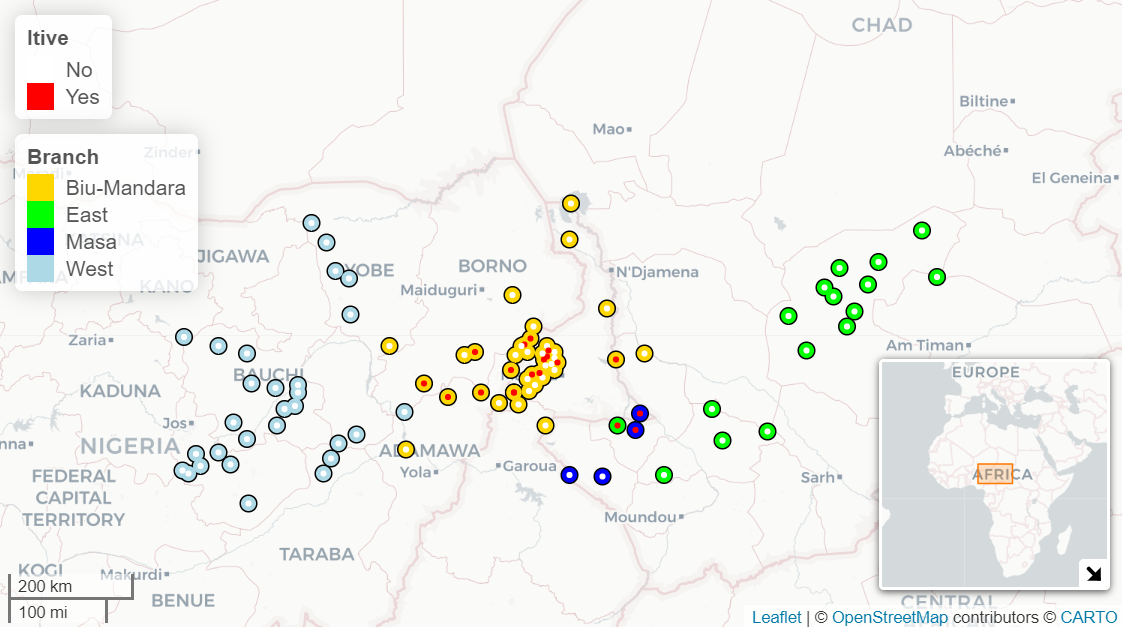
\includegraphics[width=\textwidth]{maps/itive.png}
	\caption{Map of itive extensions in Chadic by branch}
	\label{fig:itivemap}
\end{figure}

The only Chadic language outside of Biu-Mandara and Masa languages to have an itive extension is the East Chadic language \hyperref[kera]{Kera}. The morpheme \textit{-ná} is described as a counterpart of the ventive extension \textit{-dà}, but with distal meaning \citep[115]{ebertSpracheUndTradition1979}. In the few examples Ebert gives, the distal marker is either co-occurring with the totality marker \textit{wə́ra} or appears to have a postpositional function. However, in at least some contexts it is possible for \textit{-na} to appear suffixed to a verb of motion with an itive directional function, as in (\ref{ex:kera7}).  


\ea\label{ex:kera7}
\langinfo{\hyperref[kera]{Kera} verb \textit{kə́láŋ} ‘enter' with itive marker}{}{p.c., Jackie Hainaut} \\
\gll kə́láŋ-na	\\
enter-\gl{itive}	\\
\glt `went in'
\z 

%\subsection{Comparing ventive and itive extensions}

Given the complementary meanings of the itive and ventive extensions, it would be reasonable to expect some type of correlation between the presence of these two functions in particular languages. Table \ref{tab:directionals} shows that the ventive extension appears more frequently, in 47 languages, compared to the itive extension which appears in 19 languages. The higher frequency of ventive extensions follows if there is a default assumption that motion events described without a specific direction generally occur away from the deictic center \citep{wilkinsWhenGOMeans1995}, and therefore it is natural for a language to only specify ventive motion, leaving itive motion unmarked in the verbal morphology. By that line of reasoning, we would expect to find a one-way correlation such that languages are likely to have a grammaticalized ventive marker without having a grammaticalized itive marker, but not vice versa. This is, of course, the only possible pattern in West and East Chadic languages where itive extensions are absent. Among Biu-Mandara and Masa languages it is, as expected, more common to find languages with only a ventive extension than it is to find languages with only an itive extension, as shown in Figure \ref{fig:ventiveitivepie}. 17 languages have only a ventive extension with no itive extension, and 12 languages have both a ventive extension and an itive extension. However, there are six languages where an itive extension is attested, but not a ventive extension. Five of the six languages with an itive extension but no (attested) ventive extension are of the North Biu-Mandara subbranch and are geographically close to each other (\hyperref[bura]{Bura}, \hyperref[glav]{Glavda}, \hyperref[huba]{Huba}, \hyperref[marg]{Margi}, \hyperref[psik]{Psikye}).\footnote{In the case of \hyperref[psik]{Psikye}, \citet[113--114]{smithKapsikiLanguage1969} describes a verbal suffix \textit{-ke} which has a ventive subsequent motion interpretation with non-motion verbs, but no examples are given of this suffix with a motion verb. In the closely related \hyperref[bana]{Bana} language, there is a ventive extension \textit{-ke}, suggesting that Psikye likely does have a ventive extension which is yet unattested in the available data. \hyperref[gaan]{Ga'anda} is described as having an itive directional extension (and no ventive), but the same situation is found in the closely related language \hyperref[tera]{Tera} where there is enough evidence to consider the itive directional an adverb rather than a verbal extension.} In summary, it is fairly common to find an asymmetry in which languages have a ventive extension but no itive extension. The opposite asymmetry is less common.

%number in fig:ventiveitivepie are from python code in file VentItive
\begin{figure}
\begin{tikzpicture}
		\pie[radius = 1, sum = auto]{12/Both,
			17/Ventive only,
			6/Itive only,
			11/Neither}	
	\end{tikzpicture}
	\caption{Ventive and itive extensions in Biu-Mandara and Masa languages}
	\label{fig:ventiveitivepie}
\end{figure}

%\begin{figure}
%	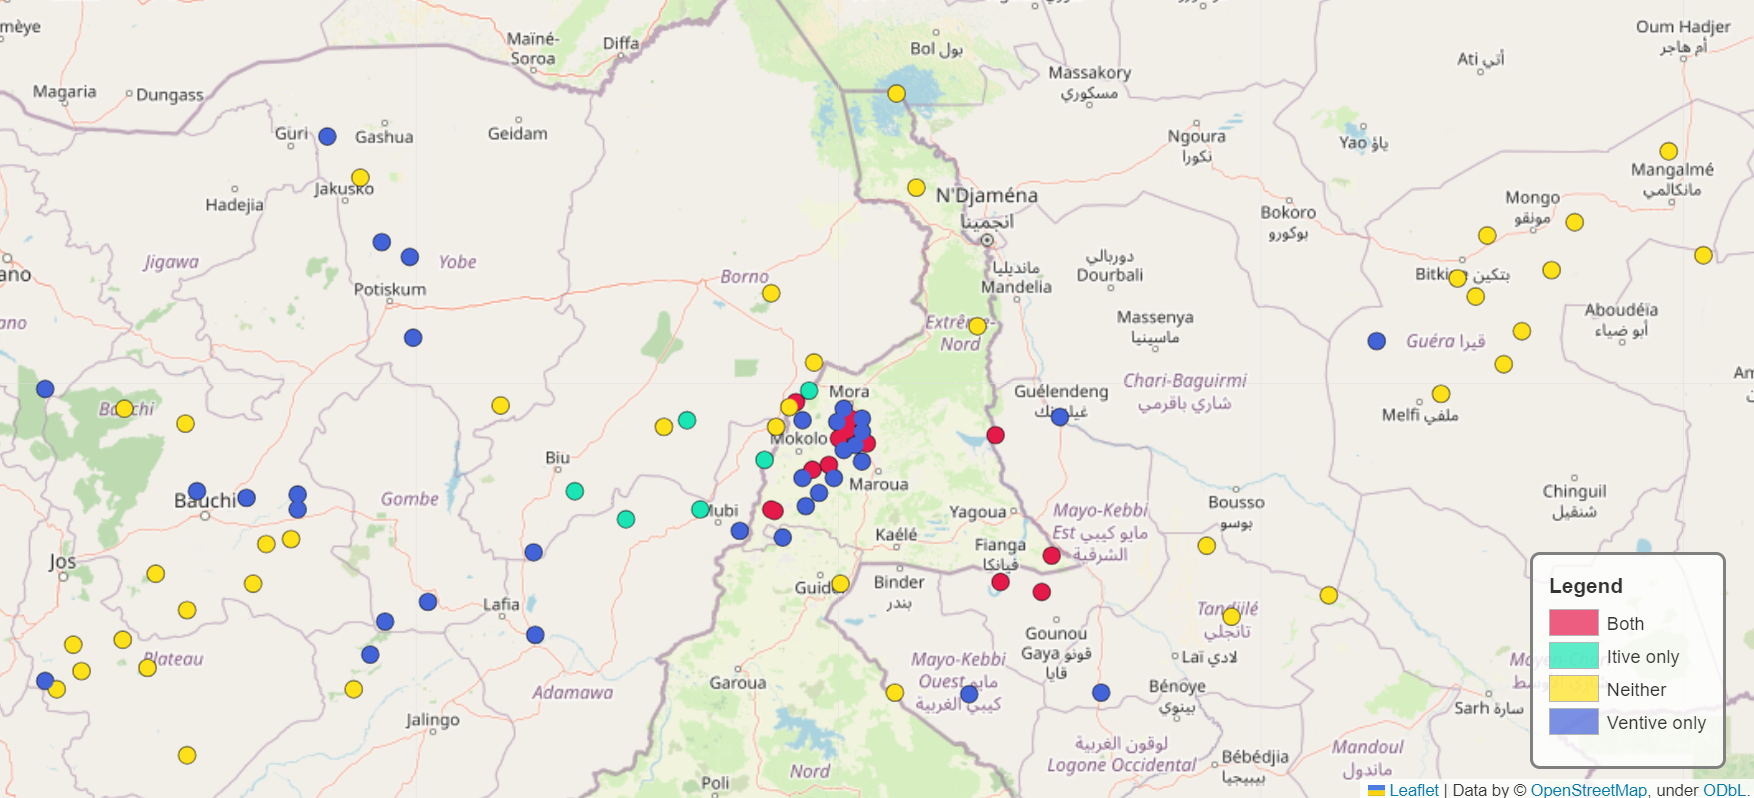
\includegraphics[width=\textwidth]{maps/ventive_itive.png}
%	\caption{Map of intersection of ventive and itive extensions in Chadic}
%	\label{fig:ventiveitivemap}
%\end{figure}	

\section{Boundary-crossing directional extensions} \label{sec:bounded2}

%\begin{figure}[h!]
%	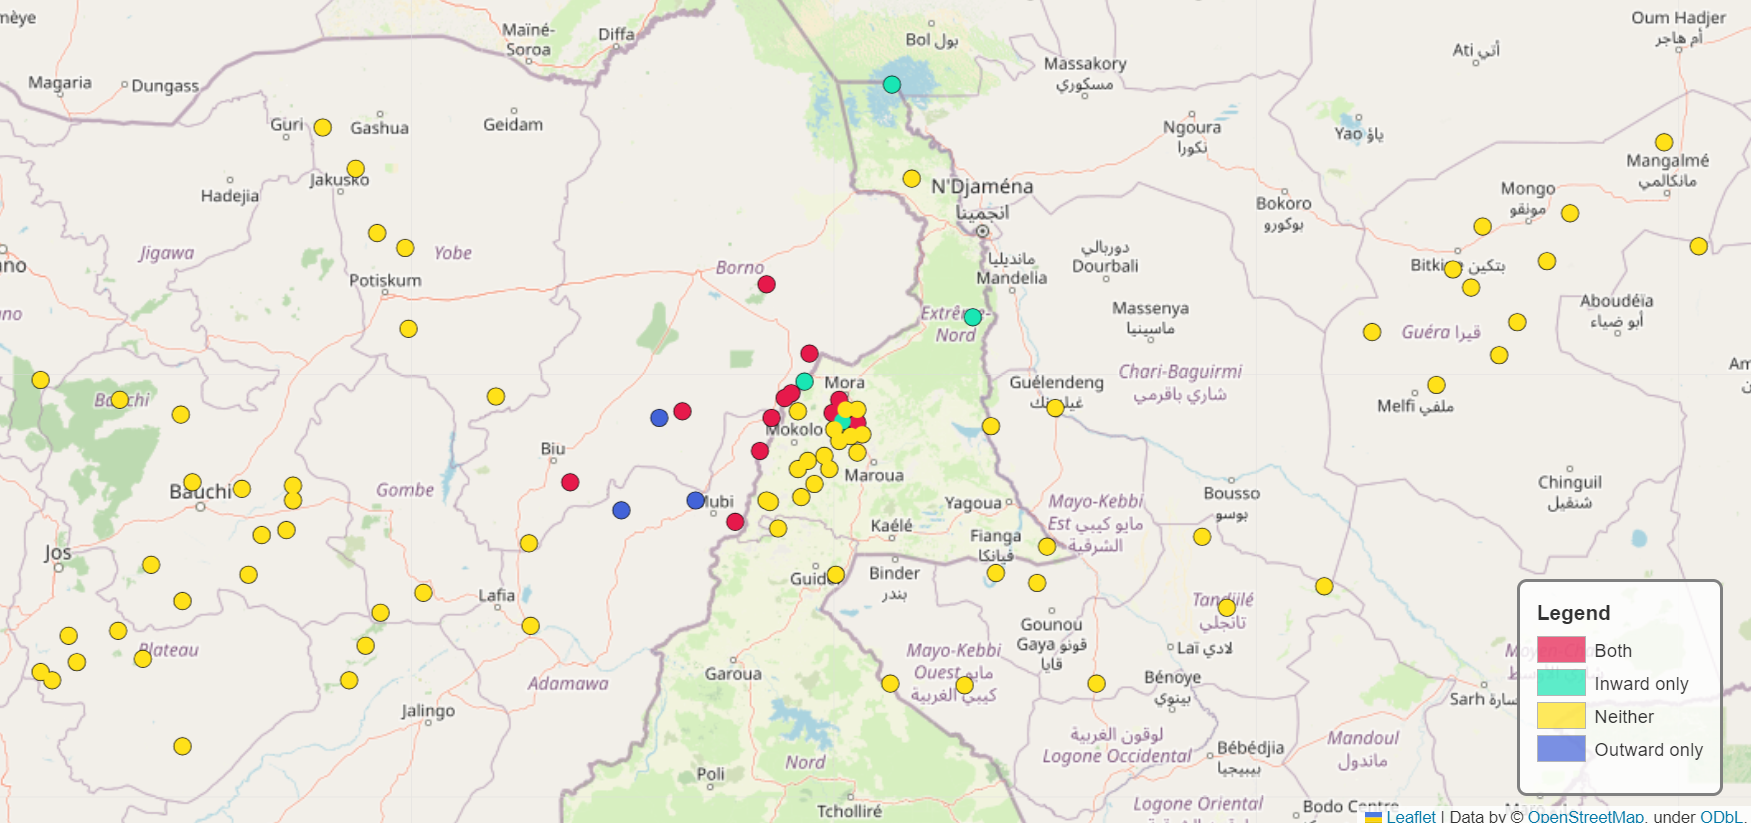
\includegraphics[width=\textwidth]{maps/in_out.png}
%	\caption{Map of boundary-crossing directional extensions in Chadic}
%	\label{fig:inoutmap}
%\end{figure}

Directional extensions expressing inward or outward motion are not as common as ventive or itive extensions. As seen in Table \ref{tab:directionals}, there are 16 languages out of the sample of 91 languages that have an inward extension, and 15 that have an outward extension. Nearly all of these languages are classified as part of the Biu-Mandara North group with only a few Biu-Mandara South languages included, as seen in Table \ref{tab:inward} and Table \ref{tab:outward}. As shown in Figure \ref{fig:inoutpie}, 12 languages have both an inward and an outward extension. Four languages only have an inward extension and three only have an outward extension. %The geographic distribution of boundary-crossing directional extensions in Chadic languages is shown on the map in Figure \ref{fig:inoutmap}.

%Data in tab:inward from python script file Inward 
\begin{table}
	\caption{Number of languages with an inward extension}
	\label{tab:inward}
	\begin{tabular}{lrrc} % add l for every additional column or remove as necessary
		\lsptoprule
		Subbranch &  Inward &  	No inward & \%\\
		\midrule
		West            &       0 &         29  &  \bwpie{0}{29} \\
%		West A            &       0 &         22  &  \bwpie{0}{22} \\
%		West B            &       0 &          7 &  \bwpie{0}{7} \\
		Biu-Mandara Hurza &       0 &          2 &   \bwpie{0}{2} \\
		Biu-Mandara North &      14 &         13 &  \bwpie{14}{13}  \\
		Biu-Mandara South &       2 &         11 &  \bwpie{2}{11} \\
		Masa 		        &       0 &         4 &  \bwpie{0}{4}  \\
%		Masa North        &       0 &         2 &  \bwpie{0}{2}  \\
%		Masa South        &       0 &          2 &   \bwpie{0}{2}  \\
		East            &       0 &          16 &   \bwpie{0}{16} \\
%		East A            &       0 &          5 &   \bwpie{0}{5} \\
%		East B            &       0 &         11 &   \bwpie{0}{11} \\
		\midrule
		Total             &      16 &         75 &   \bwpie{16}{75} \\
		\lspbottomrule
	\end{tabular}
\end{table}

%Data in tab:outward from python script file outward 
\begin{table}
	\caption{Number of languages with an outward extension}
	\label{tab:outward}
	\begin{tabular}{lrrc} % add l for every additional column or remove as necessary
		\lsptoprule
		Subbranch &  Outward &  	No outward & \%\\
		\midrule
West             &        0 &          29 &  \bwpie{0}{29} \\
%West A            &        0 &          22 &  \bwpie{0}{22} \\
%West B            &        0 &           7  &  \bwpie{0}{7} \\
Biu-Mandara Hurza &        0 &           2 &  \bwpie{0}{2} \\
Biu-Mandara North &       12 &          15 &  \bwpie{12}{15}  \\
Biu-Mandara South &        3 &          10 &   \bwpie{3}{10} \\
Masa 		        &       0 &         4 &  \bwpie{0}{4}  \\
%Masa North        &        0 &           2 &  \bwpie{0}{2}  \\
%Masa South        &        0 &           2 &  \bwpie{0}{2} \\
East             &        0 &           16 &  \bwpie{0}{16} \\
%East A            &        0 &           5 &  \bwpie{0}{5} \\
%East B            &        0 &          11 &  \bwpie{0}{11} \\
\midrule
Total             &       15 &          76 &  \bwpie{15}{76} \\
		\lspbottomrule
	\end{tabular}
\end{table}

\begin{figure}
	\begin{tikzpicture}
		\pie[radius = 1, sum = auto]{12/Both,
			4/Inward only,
			3/Outward only,
			23/Neither}	
	\end{tikzpicture}
	\caption{Boundary-crossing directional extensions in Biu-Mandara languages}
	\label{fig:inoutpie}
\end{figure}

\newpage
\section{Vertical directional extensions} \label{sec:vertical2}

As shown in Table \ref{tab:directionals}, only eight of the 91 languages in the sample have an upward extension. All of them are Biu-Mandara languages, mostly of the Biu-Mandara North subbranch, as shown in Table \ref{tab:upward}. 

%data in tab:upward from python script in file Upward
\begin{table}
	\caption{Number of Chadic languages with an upward extension}
	\label{tab:upward}
	\begin{tabular}{lrrc} % add l for every additional column or remove as necessary
		\lsptoprule
		Subbranch &  Upward &  	No upward & \% \\
		\midrule
West            &       0 &         29 &  \bwpie{0}{19} \\
%West A            &       0 &         22 &  \bwpie{0}{22} \\
%West B            &       0 &          7 &  \bwpie{0}{7} \\
Biu-Mandara Hurza &       0 &          2 &  \bwpie{0}{2} \\
Biu-Mandara North &       6 &         21 &  \bwpie{6}{21} \\
Biu-Mandara South &       2 &         11 &  \bwpie{2}{11} \\
Masa 		        &       0 &         4 &  \bwpie{0}{4}  \\
%Masa North        &       0 &         2 &  \bwpie{0}{2} \\
%Masa South        &       0 &          2 &  \bwpie{0}{2}\\
East             &         0 &            16&  \bwpie{0}{16} \\
%East A            &       0 &          5 &  \bwpie{0}{5} \\
%East B            &       0 &         11  &  \bwpie{0}{11} \\
		\midrule
Total       &     8 &       83 &  \bwpie{8}{83} \\
		\lspbottomrule
	\end{tabular}
\end{table}

A slightly higher number of languages, 13, have a downward extension. Again, all of these are Biu-Mandara languages, mostly of the Biu-Mandara North subbranch, as shown in Table \ref{tab:downward}. 

%data in tab:downward from python script in file Downward
\begin{table}
	\caption{Number of Chadic languages with a downward extension}
	\label{tab:downward}
	\begin{tabular}{lrrc} % add l for every additional column or remove as necessary
		\lsptoprule
		Branch &  Downward &  	No downward & \% \\
		\midrule
West            &       0 &         29 &  \bwpie{0}{19} \\
%West A            &         0 &           22&   \bwpie{0}{22}\\
%West B            &         0 &            7 &   \bwpie{0}{7} \\
Biu-Mandara Hurza &         0 &            2 &  \bwpie{0}{2} \\
Biu-Mandara North &        10 &           17 &  \bwpie{10}{17}\\
Biu-Mandara South &         3 &           10 &  \bwpie{3}{10} \\
Masa 		        &       0 &         4 &  \bwpie{0}{4}  \\
%Masa North        &         0 &            2 &  \bwpie{0}{2} \\
%Masa South        &         0 &            2 &  \bwpie{0}{2} \\
East             &         0 &            16&  \bwpie{0}{16} \\
%East A            &         0 &            5&  \bwpie{0}{5} \\
%East B            &         0 &           11 &  \bwpie{0}{11} \\
\midrule
Total             &        13 &           78&  \bwpie{13}{78} \\
		\lspbottomrule
	\end{tabular}
\end{table}

Chadic languages are more likely to have a downward extension without an upward extension than vice versa, as shown in Figure \ref{fig:updownpie}. Seven languages have both downward and upward extensions, six languages have only a downward extension, and just one language, \hyperref[malg]{Malgwi}, has an upward extension without also having a downward extension. 

\begin{figure}
	\begin{tikzpicture}
	\pie[radius = 1, sum = auto]{7/Both,
		1/Upward only,
		6/Downward only}	
\end{tikzpicture}
	\caption{Chadic languages with upward and/or downward extensions}
	\label{fig:updownpie}
\end{figure}

%The geographic distribution of vertical extensions is shown in Figure \ref{fig:updownmap}. 
Languages with vertical extensions are clustered around the Nigeria-Came\-roon border, precisely where the Mandara mountain range is located. While the correlation between vertical extensions and a mountainous environment is striking, it should be emphasized that other Chadic languages are spoken in mountainous areas without having developed any vertical directional extensions. The mountains of the Guera Massif in central Chad, where many East Chadic languages are spoken, and the Jos Plateau, where many West Chadic languages are spoken, are of similar elevation to the Mandara mountains.

%\begin{figure}
%	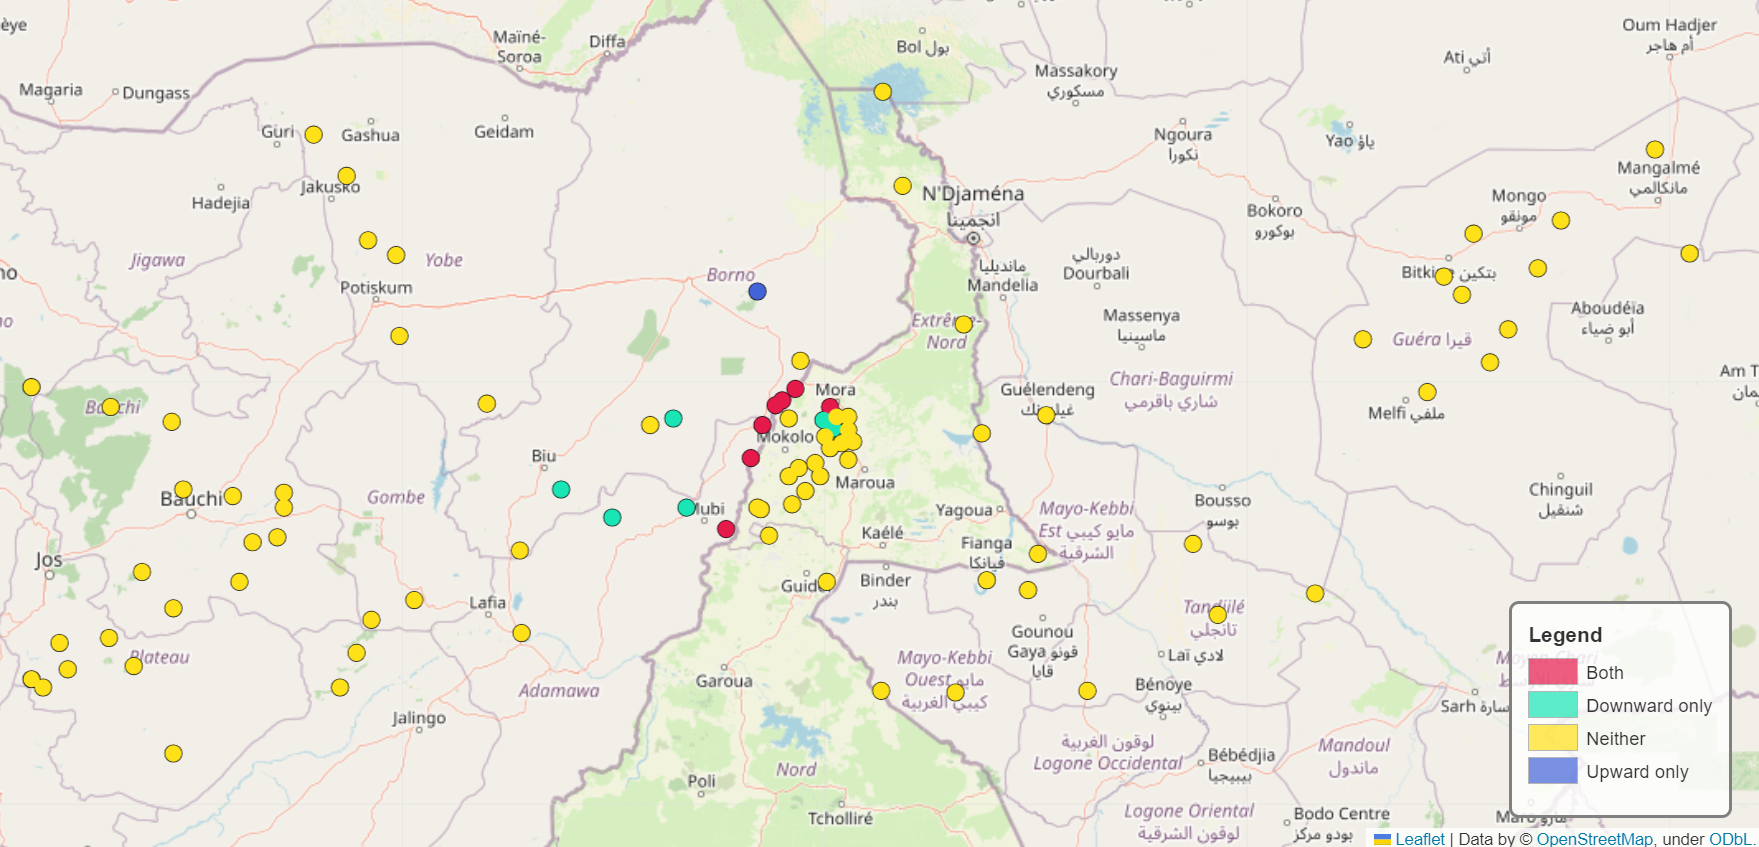
\includegraphics[width=\textwidth]{maps/up_down.png}
%	\caption{Map of upward and downward extensions in Chadic}
%	\label{fig:updownmap}
%\end{figure}

\section{Directional extensions `onto' and `under'}  \label{sec:onto2}

There are nine languages with an `onto' directional extension, as indicated in Table \ref{tab:directionals} above. All nine of these languages are in the Biu-Mandara North subbranch, and all but one are in the Margi-Mandara-Mofu group. The three languages with an `under' directional extensions are all Mandaraic languages (Biu-Mandara North). The forms of these extensions, shown in Table \ref{tab:under}, all share a segment \textit{s}, suggesting that they are cognate forms (Chapter \ref{ch:diachrony}).

%The geographic distribution of the nine languages with an `onto' extension is shown in Figure \ref{fig:ontomap}.

%\begin{figure}
%	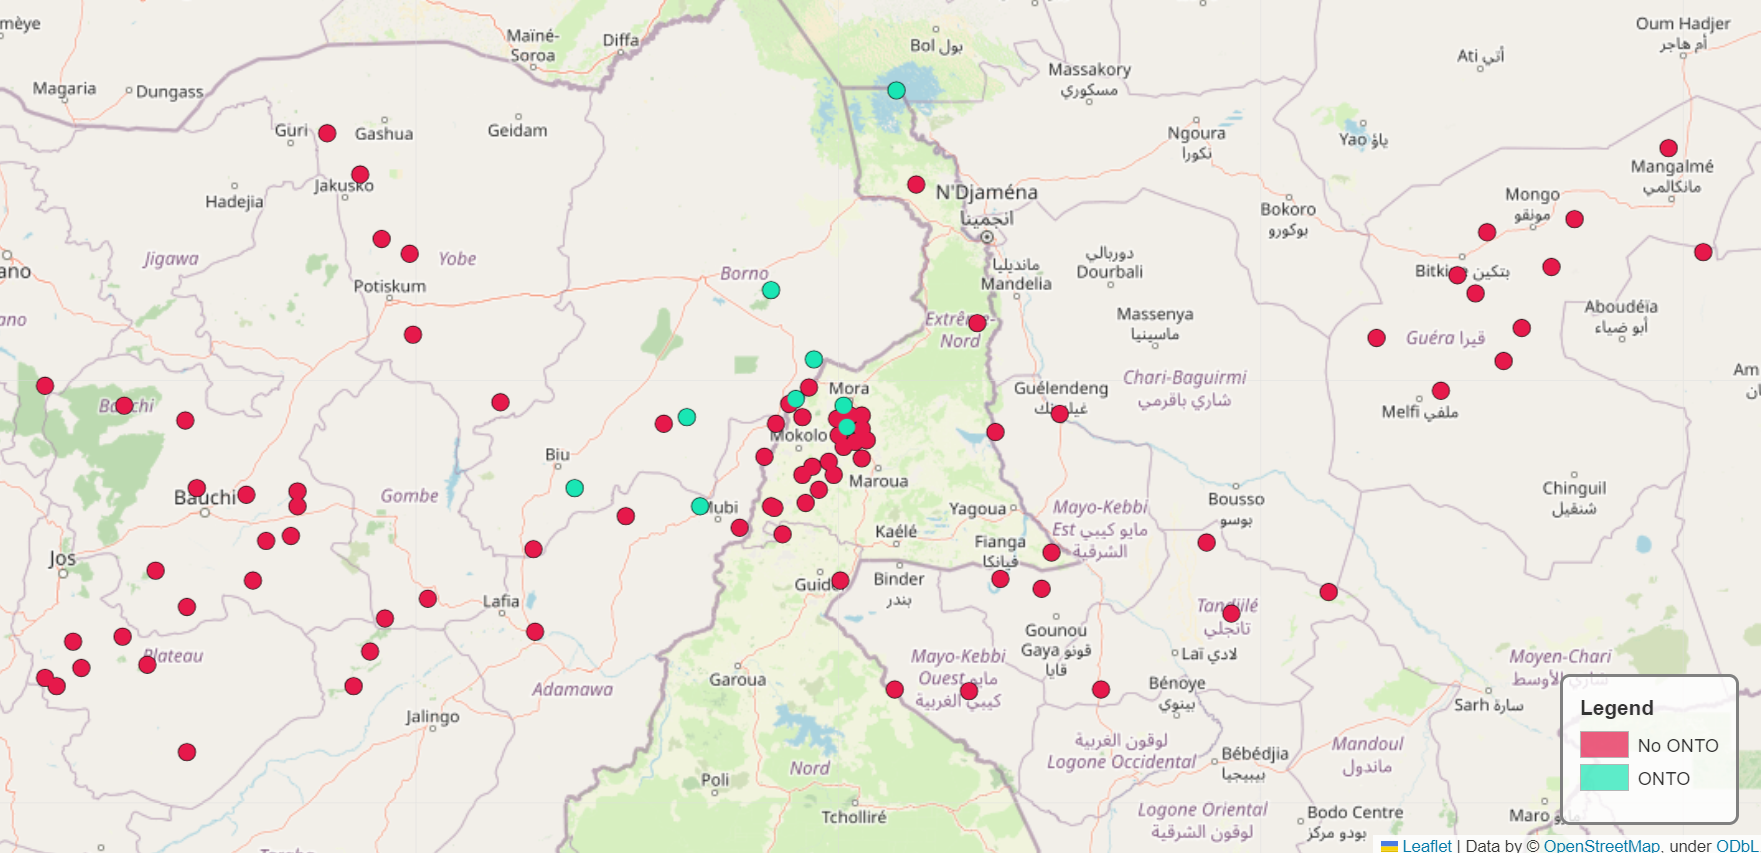
\includegraphics[width=\textwidth]{maps/onto.png}
%	\caption{Map of `onto' extensions in Chadic}
%	\label{fig:ontomap}
%\end{figure}

\begin{table}
	\caption{Forms of `under' extensions in Mandaraic subgroup}
	\label{tab:under}
	\begin{tabular}{ll}
		\lsptoprule
	Language	&     Form    \\ %&  Group & Subgroup         \\
		\midrule
%		\hyperref[bura]{Bura} & \textit{kəra}, \textit{nkir} ? & M.-M.-M. & Bura-Margi \\
		\hyperref[dghw]{Dghwede} & \textit{sege} \\ %& Margi-Mandara-Mofu & Mandaraic \\
		\hyperref[park]{Parkwa}	 & \textit{asə} \\ %& M.-M.-M. & Mandaraic \\
		\hyperref[glav]{Glavda} &	\textit{s}	\\ %&	M.-M.-M.	& Mandaraic \\	
		\lspbottomrule
	\end{tabular}
\end{table}

\section{Co-occurrence of directional extensions in particular languages} \label{sec:co-occurrence}

The above sections examined how frequently each particular semantic type of directional extension is attested across a sample of Chadic languages. This section looks at how many semantic types of directional extensions co-occur in a particular language. The directional meanings considered are the eight discussed in the above sections.\footnote{If including the more rarely attested semantic types, \hyperref[psik]{Psikye} also has a bushward extension bringing its total up from five to six, \hyperref[lama]{Lamang} also has a homeward extension bringing its total up from four to five, and Bura has both a homeward and a `side' extension bringing its total up from five to seven. } The number in the first column of Table \ref{tab:multiple} is the number of these eight directional meanings that are expressed through a verbal extension in a particular language, from zero up to eight. The remaining columns indicate how many languages of each branch of Chadic languages have that number of directional meanings attested in verbal extensions.\footnote{A direct comparison of Table \ref{tab:multiple} with Table \ref{tab:dirmorphs} shows a discrepancy in the row labeled `1'. This is because \hyperref[kana]{Kanakuru} has two directional extensions (post-verbal \textit{-tə(ru)} and pre-verbal \textit{bo}) which are each counted as separate morphemes in Table \ref{tab:dirmorphs}, but both directional extensions express the same meaning, ventive, and so are only counted once in Table \ref{tab:multiple} which tabulates how many of the main eight types of directional meaning each language can express.} 

%Data in tab:multiple is from python script in Number file 
\begin{table}
	\caption{Number of directional meanings expressed}
	\label{tab:multiple}
	\begin{tabular}{rrrrrc}
		\lsptoprule
{} &  West &  Biu-Mandara &  Masa &  East &  Total \\
\midrule
0 &    14 &            3 &     1 &    13 &     31 \\
1 &    15 &           14 &     1 &     2 &     32 \\
2 &     0 &            9 &     2 &     1 &     12 \\
3 &     0 &            3 &     0 &     0 &      3 \\
4 &     0 &            5 &     0 &     0 &      5 \\
5 &     0 &            6 &     0 &     0 &      6 \\
6 &     0 &            0 &     0 &     0 &      0 \\
7 &     0 &            1 &     0 &     0 &      1 \\
8 &     0 &            1 &     0 &     0 &      1 \\
%Including SIDE, BUSH, HOME
%0 &    15 &            3 &     1 &    13 &     32 \\
%1 &    14 &           14 &     1 &     2 &     31 \\
%2 &     0 &            9 &     2 &     1 &     12 \\
%3 &     0 &            3 &     0 &     0 &      3 \\
%4 &     0 &            4 &     0 &     0 &      4 \\
%5 &     0 &            5 &     0 &     0 &      5 \\
%6 &     0 &            1 &     0 &     0 &      1 \\
%7 &     0 &            2 &     0 &     0 &      2 \\
%8 &     0 &            1 &     0 &     0 &      1 \\
		\lspbottomrule
	\end{tabular}
\end{table}

Over half of the languages with a directional extension (32 of 60) have only one of the eight main semantic types of directional extension, as seen in Figure \ref{fig:multiple}. All but two of these are languages with a ventive directional extension. The others are \hyperref[lagw]{Lagwan} (only inward) and \hyperref[ciba]{Cibak} (only outward).\footnote{In a description of \hyperref[ciba]{Cibak}, \citet{hoffmannZurSpracheCibak1955} mentions a second directional extension, \textit{-nta}. However, the examples given do not substantiate the putative itive directional meaning of this extension.} Twelve languages have two types of directional extensions. Nearly all of these include ventive and itive directional meaning with the sole exception of \hyperref[budu]{Buduma} (inward and `onto'). 

\begin{figure}
	\begin{tikzpicture}
	\pie[radius = 3, sum = auto]{
		32/One,
		12/Two,
		3/Three,
		5/Four,
		6/Five,
		1/Seven,
		1/Eight}	
\end{tikzpicture}
	\caption{Number of directional meanings expressed in verbal extensions}
	\label{fig:multiple}
\end{figure}

In the 16 languages with more than two directional extensions, the ventive type is much less common. Only six of these 16 languages have a ventive extension. In languages with just one or two directional extensions, the ventive appears in 41 of 44 cases. Therefore, there is no implicational hierarchy such that the presence of one type of directional extension entails the existence of another type in the same language (at least from a synchronic perspective). 

Why are ventive extensions ubiquitous in languages with just one or two directional extensions, and much less common in languages with more than two directional extensions? One potential explanation for this pattern may be that there are cognitive motivations for not needing a ventive marker in a more complex system of directional extensions. The other directional extensions provide a rich set of directional notions that render the ventive meaning superfluous. Alternatively, from a diachronic perspective, it could be hypothesized that languages with more directional extensions have developed over an extended period of time, and that during this timespan erstwhile ventive directional extensions have shifted to another function. 

The hypothesis that some ventive forms have undergone reanalysis would be supported if languages without ventive extensions can be shown to have cognate extensions with other functions. For example, \hyperref[bura]{Bura} and \hyperref[marg]{Margi} are languages with multiple directional extensions but no ventive extension. Both languages have an inward extension of the form \textit{-wa}. Could this inward extension be historically related to the ventive extension \textit{-awa} found in other languages of the same subgroup of Margi-Mandara-Mofu languages? More historical reconstruction of each subgroup would be needed to substantiate these types of cognate relationships.

Whereas ventive directional meaning is less common in languages with more directional extensions, conversely, the rarest types of directional extensions (`under', homeward, bushward) are only attested in languages with at least four other types of directional extensions. Diachronically, this suggests that these semantic types have only developed as verbal extensions in languages which already have a robust system of directional extensions including at least some of the inward, outward, upward or downward directional extensions. 

\section{Conclusion} \label{sec:sumdir}

\citet[148]{creisselsAfricaMorphosyntacticArea2008} report that directional morphemes attached to the verb ``are not very common in African languages in general, but they are common in Nilo-Saharan languages.'' While not all verbal extensions in Chadic languages are affixes, it is still reasonable to say that directional verbal morphology is also common in Chadic languages, as the majority of Chadic languages have at least one verbal extension with a directional function, of which most are suffixes. 

The most common directional meaning among Chadic verbal extensions is ventive, toward the deictic center. This is the only type of directional meaning found in verbal extensions across all four branches of Chadic languages. Ventive directionals are also commonly found in the more distantly related Berber languages \citep{mettouchiGrammaticalizationDirectionalClitics2011}. Biu-Mandara languages have innovated beyond ventive meaning and added several other types of directional meaning to their inventory of verbal extensions. Most often, the meanings added are itive, inward, outward, upward and downward. In a global sample of directional morphemes in 114 languages, Ross finds ventive, itive, upward and downward motion to be the most common semantic types. Vertical directional extensions are found in 14 Chadic languages out of 59 Chadic languages with directional extensions (24\%). This is significantly lower than the global average from Ross' sample in which vertical directional semantics are found in 50 of 114 languages with directional morphemes (44\%).\footnote{By binomial test, the rate of 14 of 59 is significantly lower than the rate of 44\% in Ross' sample (p < 0.001). \citet[279]{rossPseudocoordinationSerialVerb2021} also examines the linear order of directional verbal morphology and the verb it modifies. The results are that directional morphology is post-verbal in 59\% of the sample. All directional morphology in Chadic languages is post-verbal with the exception of the \hyperref[kana]{Kanakuru} auxiliary \textit{bo} \citep[76]{newmanKanakuruLanguage1974}.} In Chadic languages that have multiple directional extensions, less common directional meanings are found, such as `onto' and `under', as well as homeward and bushward. This matches the global pattern in which less common types of directional meaning typically occur in languages that have a larger number of directional morphemes \citep[278]{rossPseudocoordinationSerialVerb2021}. 

\citet{bickelTypology21stCentury2007} describes linguistic typology as answering the multipart question ``What’s where why?'' As summarized above, this chapter has provided a robust response to the \textit{what} and \textit{where} questions of directional extensions in Chadic languages. Answering the \textit{why} question is an even more challenging task, and it ultimately cannot be fully addressed without expanding beyond Chadic languages to examine the genetic context of Afro-Asiatic languages and the areal context of the highly multilingual and linguistically diverse environments in which the Chadic languages are spoken. One step toward that goal in future research will be to construct a theory of \textit{how} Chadic languages came to be the way they are in the sense of understanding what the major processes of historical change have been. A historical reconstruction is not the main goal of this research, but the available evidence gleaned from the comparative synchronic picture is presented in Chapter \ref{ch:diachrony} awaiting further investigation when possible. 
